\section{Optimization}

Human vision has noticeable thresholds for the perception of light frequency. We are a lot more sensitive to lower frequencies compared to higher ones. JPEG image compression involves identifying high frequency pixel groupings and removing them from the image; less data in the image matrix means that it takes up less digital storage.  We can compress the image by using the DST to identify high frequency data. We can also vary the extent of compression using a variable “$p$,” which goes from 0 to 1 where 0 represents a blank image and 1 represents an uncompressed image. To see a demonstration of how different values of $p$ affect the image's quality, please either click \framebox{\href{http://will-farmer.com/diffeq/Project_2_matrices/img/comp1.gif}{this link}} or download it \attachfile{./img/comp1.gif}{here}.

Because our equation focusses only on the high frequency values of the image, we can eliminate many pixels before our brains register a degradation in quality. Below is a graph that shows how much data is removed from each image as $p$ gets larger.

    \begin{figure}[ht]
        \centering
        \begin{subfigure}{0.41\textwidth}
            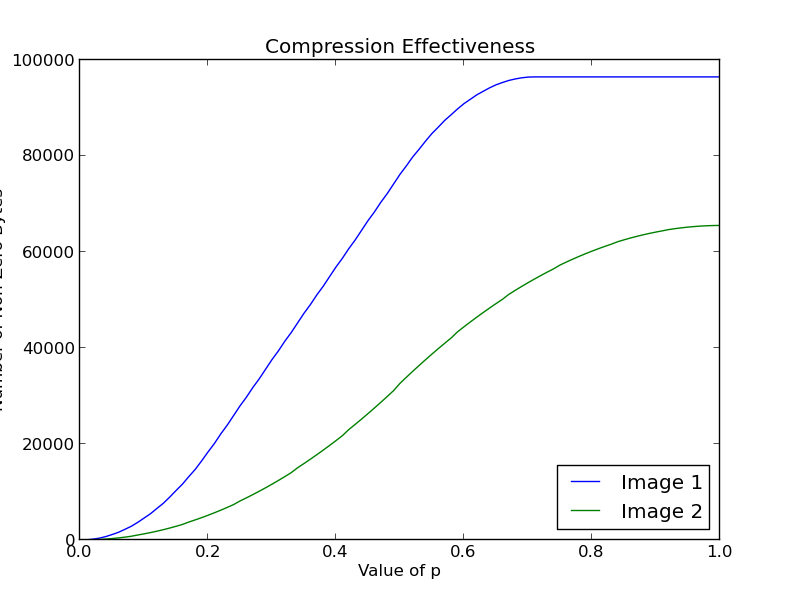
\includegraphics[scale=0.35]{./img/bitcount.png}
            \label{fig:bitcount}
            \caption{Bit Count vs. $p$ Value}
        \end{subfigure}
        \begin{subfigure}{0.41\textwidth}
            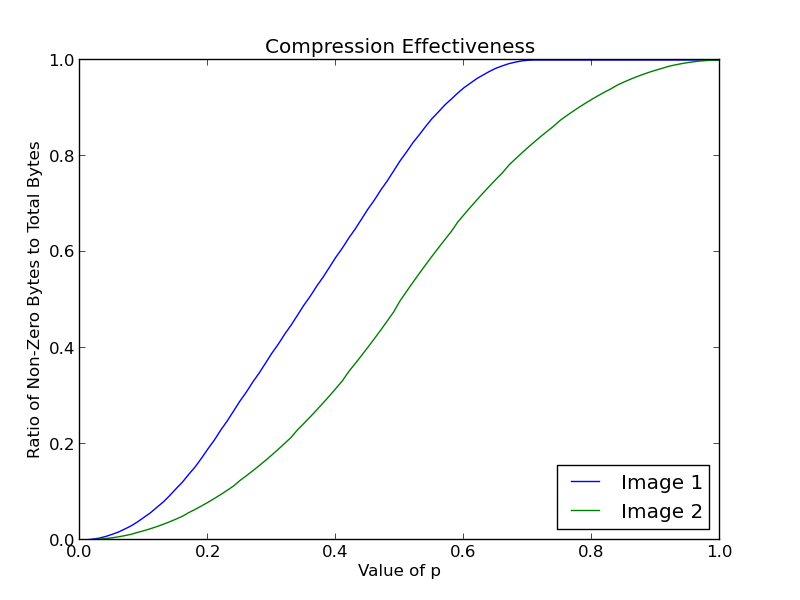
\includegraphics[scale=0.35]{./img/bitrat.png}
            \label{fig:bitrat}
            \caption{Bit Ratio vs. $p$ Value}
        \end{subfigure}
        \label{figs:bits}
    \end{figure}

Images can be compressed to low values of $p$ without being noticeable, especially if the images are primarily uniform and consist of low frequency pixels. This is because of the threshold frequencies in human vision.

Due to the inherent nature of images having different amounts of high frequency values, different values of $p$ will be appropriate for different images. For our first image, it initially will not have a large difference in quality as $p$ gets smaller, however for our last image it will immediately start reducing in size. Therefore different values of $P$ are appropriate for these different images.
